\section{UML-based Specification Environment (USE)}

\subsection{Overview}
The UML-based Specification Environment (USE) is a system for the specification and 
validation of information systems based on a subset of UML and OCL \cite{USE}. 
Models in USE are specified in textual form (as .use files) containing classes with 
their attributes and operations, associations, and OCL constraints. These constraints 
include class invariants and operation pre/postconditions, all defined using OCL 
expressions. USE supports model animation to validate specifications against 
non-formal requirements, allowing developers to create and manipulate system states 
(snapshots) during animation. For each snapshot, USE automatically checks OCL 
constraints and highlights violations. The tool provides comprehensive graphical 
visualization of model elements through various diagram types, including class 
diagrams, object diagrams, and sequence diagrams. Additionally, USE allows users 
to enter and evaluate OCL expressions interactively to query detailed information 
about the current system state. This combination of precise specification with 
dynamic validation makes USE particularly valuable for detecting inconsistencies 
and design flaws early in the development process. Figure \ref{fig:use_overview}
gives a general view of the USE approach.

\begin{figure}
    \centering
    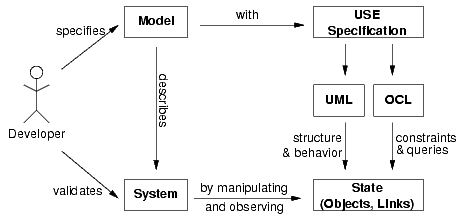
\includegraphics[width=0.8\textwidth]{figures/c1/USE_Overview.png}
    \caption{USE Overview.}
    \label{fig:use_overview}
\end{figure}

\subsection{USE Model Validator}
The Model Validator extends USE's capabilities through a specialized plugin that 
automates the generation of object diagrams from class diagrams within a configurable 
search space \cite{USE}. This plugin bridges the gap between manual model animation 
and systematic verification by employing a transformation-based approach. The 
validator converts UML/OCL models into relational logic using Kodkod \cite{Kodkod}, which is 
subsequently transformed into a boolean satisfiability (SAT) problem for efficient 
analysis. When a solution is found, it is immediately displayed as an object diagram 
in the USE interface, with the option to explore alternative valid states \cite{Model_Validator_2}. Developers 
control the validation process through configuration files (.properties) that define 
search parameters, including upper and lower bounds for classes, attributes, and 
associations. These configurations can be supplemented with additional OCL invariants 
to target specific scenarios \cite{Properties_file}. When executed via the validate command, the Model 
Validator systematically searches for system states that satisfy all constraints, 
reporting either SATISFIABLE (with a corresponding object diagram) when a valid 
configuration exists, or UNSATISFIABLE when the constraints cannot be collectively 
satisfied. This automated approach significantly enhances USE's ability to detect 
inconsistencies and validate model properties that would be difficult to verify 
through manual testing alone.


\subsection{Filmstripping}
\label{subsec:filmstripping}
\subsubsection{Overview}
Filmstripping is a model transformation technique developed to extend USE's 
verification capabilities from static structure to dynamic behavior \cite{AM2Filmstrip} \cite{Filmstripping}. 
While standard OCL validation tools (including USE's Model Validator) primarily 
focus on structural aspects like invariants, the filmstrip approach enables 
verification of behavioral properties by transforming dynamic specifications into 
static ones. The method works by converting a UML/OCL model containing both invariants 
and operation pre/postconditions into an equivalent model containing only invariants. 
This transformed "filmstrip model" consists of the original application model 
augmented with specialized structures that capture system state progression. The 
key insight is the introduction of explicit \texttt{Snapshot} classes that represent 
individual system states, with \texttt{OperationCall} classes that connect 
consecutive snapshots. Through this transformation, temporal sequences of operations 
and object states are flattened into a single, verifiable object diagram. Pre and 
postconditions from the original model are systematically converted into invariants 
that constrain relationships between snapshots, effectively embedding behavioral 
specifications within the static structure. This approach enables the Model Validator 
to verify complex behavioral properties—including operation sequencing, state 
transitions, and temporal constraints—using the same validation mechanisms originally 
designed for structural verification. By bridging the gap between static and dynamic 
validation, filmstripping provides a comprehensive framework for verifying both 
aspects of a model within a single technical infrastructure. In the following 
subsection, we detail the specific transformation process that converts standard 
UML/OCL models into filmstrip models, explaining how operation contracts are 
transformed into invariants and how system state progression is represented.

\subsubsection{Filmstrip Model Transformation}

\begin{figure}
    \centering
    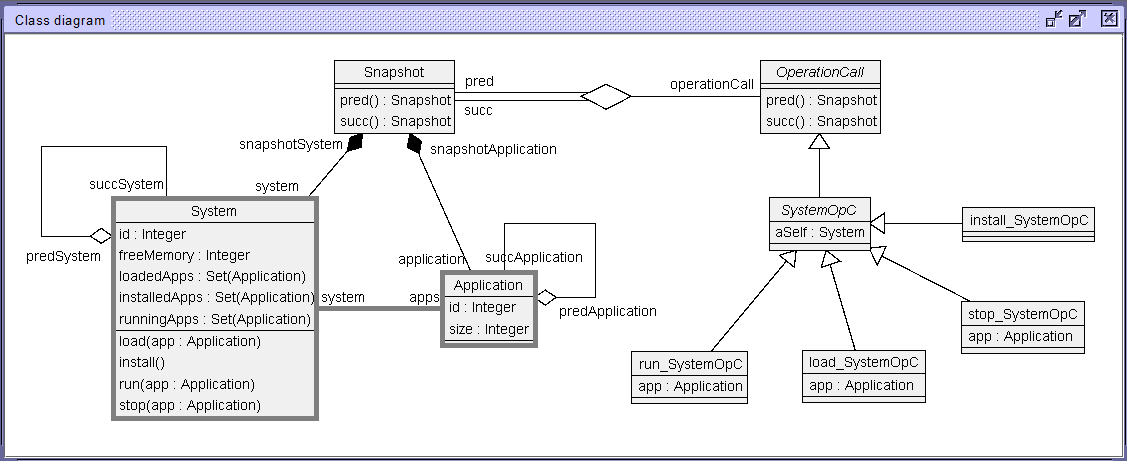
\includegraphics[width=1\textwidth]{figures/c1/SoftwareSystem/SS_Filmstrip_Gray_Edited.png}
    \caption{Filmstrip Model Transformation.}
    \label{fig:filmstrip_model}
\end{figure}

The filmstrip transformation process is best illustrated through an example. 
Figure \ref{fig:filmstrip_model} shows the transformation of our Software System 
model from Figure \ref{fig:class_diagram_software_system} into its filmstrip 
equivalent. The original application model—classes \texttt{System} and 
\texttt{Application} with their \texttt{SystemApplication} association—remains 
intact within the filmstrip model, visually distinguished by gray borders.

The transformation is performed automatically by the Filmstrip Plugin for USE \cite{Filmstripping}, which 
augments the original model with additional elements (shown without gray borders). 
These elements include \texttt{Snapshot} objects that capture individual system 
states and \texttt{OperationCall} classes (with suffix \texttt{OpC}) that represent 
the operations from the application model. Each operation is converted into a 
corresponding \texttt{OperationCall} class containing attributes for the context 
object (self) and operation parameters.

The complete transformation process involves the following steps \cite{Filmstripping}:
\vspace{-1.2em}
\paragraph{Transformation of classes:} All classes and attributes from the 
application model are preserved in the filmstrip model. Two essential classes are 
added: \texttt{Snapshot}, which associates objects with specific system states, 
and \texttt{OperationCall}, which represents state transitions. Operation parameters 
become attributes in their respective operation call classes, and all operation call 
classes inherit from the base \texttt{OperationCall} class through generalization.
\vspace{-1.2em}
\paragraph{Transformation of associations:} All original associations are maintained 
in the filmstrip model. A crucial ternary association is added to link pre-snapshots 
to post-snapshots through operation calls, representing the system's state evolution. 
Additional associations connect application objects to their respective snapshots, 
ensuring that each object exists in exactly one snapshot state, while aggregation 
links represent object persistence across snapshots.
\vspace{-1.2em}
\paragraph{Transformation of operation definitions and invariants:} Operation 
definitions and invariants from the application model are incorporated without 
modification.
\vspace{-1.2em}
\paragraph{Transformation of pre- and postconditions:} Operation contracts (pre- and 
postconditions) are converted into invariants in the filmstrip model, associated with 
their respective operation call classes. These invariants are evaluated once for each 
operation call instance, preserving the semantic equivalence between the original 
contracts and their filmstrip representations.

